\chapter{Integrali Doppi}\label{chap:int_doppi}
Il presente capitolo non è trattato in maniera approfondita poiché:
\begin{itemize}
	\item Sarebbero necessari molti lunghi teoremi per poter introdurre rigorosamente la teoria di Riemann, inoltre sarebbero fuori contesto nel corso.
	\item La teoria di Riemann è "superata" da tempo.\\
		Il primo è più grosso problema di tale teoria è che non permette il passaggio del limite sotto il segno di integrale, cioè per poter scrivere 
		\[ \int\lim\limits_{n\to\infty}f_n(x) = \lim\limits_{n\to\infty}\int f_n(x)\]
		sono necessarie molte ipotesi restrittive.
\end{itemize}
Per queste ragioni nell'Analisi è passati alla teoria dell'integrale secondo Lebesgue, molto diversa e piuttosto complicata.
\begin{figure}[H]
	\centering
	% Thanks to https://it.wikipedia.org/wiki/File:RandLintegrals.svg
	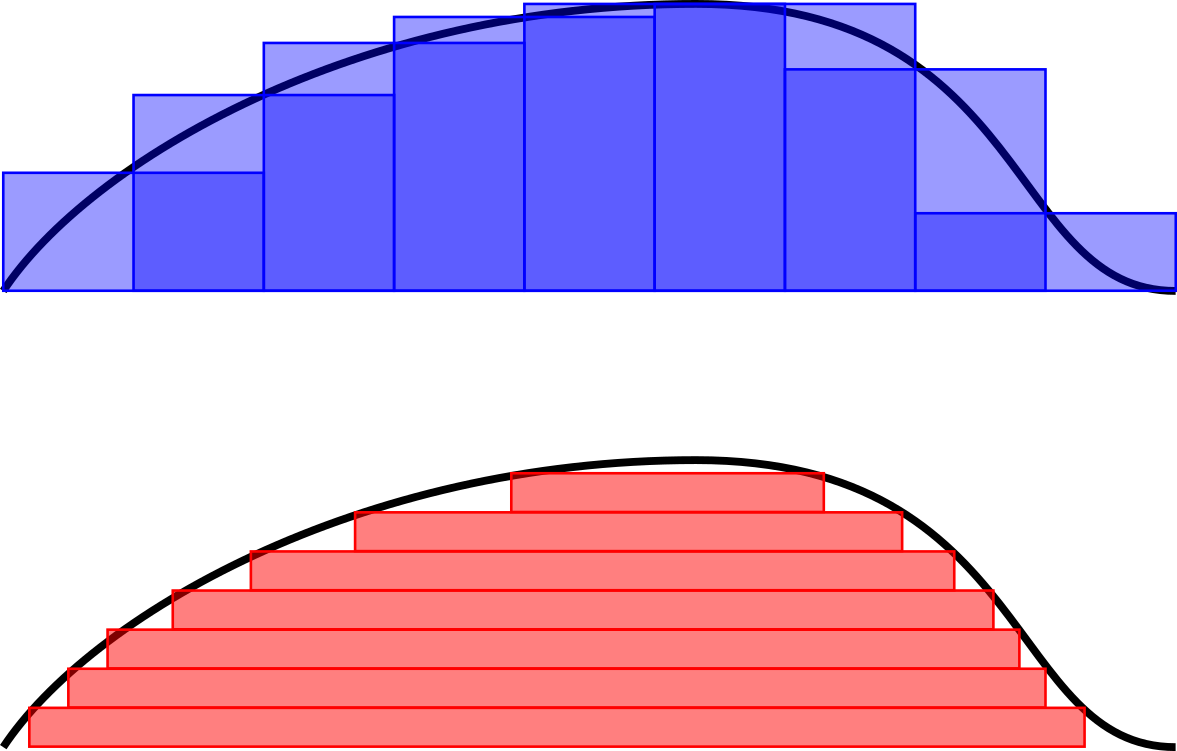
\includegraphics[width=.4\linewidth]{2d-riemann-lebesgue-integral}
	\caption{Sopra, integrale di Riemann\\Sotto, integrale di Lebesgue}
\end{figure}

Il concetto di Integrale è quindi molto legato ad area e volume. La teoria di Lebesgue riparte da assiomi come questi definendoli e caratterizzandoli per in maniera sistematica e rigorosa cosa si possa e cosa non si possa integrare e dove abbia senso parlare di superfici, volumi, ipervolumi\dots

\newpage
\section{Regole di Calcolo}
Le seguenti formule permettono di ricondurre il calcolo di integrali doppi a quello di integrali semplici.

\begin{figure}[H]
	\centering
	% The two graphs are placed in the same tikz env to avoid issues with axis alignment
	\begin{tikzpicture}
		% First graph
		\draw[->] (0,0) -- (5.5,0) node[anchor=north west] {$x$};
		\draw[->] (0,0) -- (0,4) node[anchor=south east] {$y$};
		\draw[dotted] (.5,0) node[below] {$a$} -- (.5,4) ;
		\draw[dotted] (4,0) node[below] {$b$} -- (4,4);
		\draw[domain=.5:4, smooth, variable=\x] plot ({\x},{(1/10)*(\x*\x*\x) - (\x/2+2)*(\x/2+2) + 1.5*\x + 7}) node[left, xshift=-25, yshift=-32] {$y=\beta(x)$};
		\draw[domain=.5:4, smooth, variable=\x] plot ({\x},{(1/15)*\x*\x + (1/10)*cos(2*\x r) + 0.5}) node[left, yshift=-25] {$y=\alpha(x)$};
		\node at (1.5, 1.3) {$A$};
		% Second graph
		\draw[->] (8,0) -- (13.5,0) node[anchor=north west] {$x$};
		\draw[->] (8,0) -- (8,4) node[anchor=south east] {$y$};
		\draw[dotted] (8,.5) node[left] {$c$} -- (12,.5);
		\draw[dotted] (8,3.5) node[left] {$d$} -- (12,3.5);
		\draw[domain=.5:3.5, smooth, variable=\y] plot ({8 + sin(\y r) + 3}, {\y}) node[right, xshift=17, yshift=-10] {$x=\gamma(y)$};
		\draw[domain=.5:3.5, smooth, variable=\y] plot ({8 + (1/15)*\y*\y + (1/10)*cos(2*\y r) + 0.5},{\y}) node[yshift=-75] {$x=\delta(y)$};
		\node at (10.2, 2) {$A$};
	\end{tikzpicture}
	\caption{Integrali doppi}
	\label{fig:int_dopp}
\end{figure}
\noindent Se si è nel caso di \autoref{fig:int_dopp} a sinistra, cioè:
\begin{align*}
	a, b \quad &\in \quad \R, \quad a < b\\
	\alpha, \beta \quad &\in \quad \cntclass{0}\bigl( \intervalclose{a}{b}, \R \bigr), \quad \forall x \in \intervalclose{a}{b}\; \alpha(x) \leq \beta(x)\\
	A \quad &= \quad \brackets{(x,y) \in \R^2: \quad x \in \intervalclose{a}{b} \;\; \text{e} \;\; y \in \intervalclose{\alpha(x)}{\beta(x)}}\\
	f \quad &\in \quad \cntclass{0}(A, \R)
\end{align*}
allora
\[\iint_A f(x,y) \integrald{x} \integrald{y} = \int_a^b \left( \int_{\alpha(x)}^{\beta(x)} f(x,y) \integrald{y} \right) \integrald{x}\]

\vspace*{\baselineskip}
\noindent Se invece si è nel caso di \autoref{fig:int_dopp} a destra, cioè:
\begin{align*}
	c, d &\in \R, \quad c < d\\
	\gamma, \delta &\in \cntclass{0}\bigl( \intervalclose{c}{d}, \R \bigr), \quad \forall y \in \intervalclose{c}{d}\; \gamma(y) \leq \delta(y)\\
	A &= \brackets{(x,y) \in \R^2: \quad y \in \intervalclose{c}{d} \;\; \text{e} \;\; x \in \intervalclose{\gamma(y)}{\delta(y)}}\\
	f &\in \cntclass{0}(A, \R)\\
\end{align*}
allora
\[\iint_A f(x,y) \integrald{x} \integrald{y} = \int_c^d \left( \int_{\gamma(y)}^{\delta(y)} f(x,y) \integrald{x} \right) \integrald{y}\]
Quando entrambe le formule possono essere applicate, esse danno lo stesso risultato.
\begin{note}
	Integrali su regioni più complicate possono essere calcolati suddividendo opportunamente il dominio di integrazione ed usando l'addittività rispetto all'insieme su cui si integra.	
\end{note}

\newpage
\section{Cambiamento di Variabili}
Spesso può essere comodo eseguire un cambiamento delle variabili per calcolare integrali
\begin{proposition}
	Se:
	\begin{align*}
		A \quad &\subseteq \quad \R^2\\
		\Phi \quad &\in \quad \cntclass{1}(A; \R^2)\\
		\Phi  \quad &\;\,\text{è} \quad \;\,\text{\textbf{Invertibile}}\\
		\Phi^{-1}  \quad &\in \quad \cntclass{1}\left( \Phi(A);\R^2 \right)\\
		\det D\Phi \quad &\neq \quad 0 \text{ su } A\\
		f \quad &\in \quad \cntclass{0}\left( \Phi(A);\R^2 \right)
	\end{align*}
	Allora:
	\[ \iint_{\Phi(A)} f(x,y) \integrald{x} \integrald{y} = \iint_A \bigl( (f \circ \Phi)(u,v) \bigr) \abs{\det D\Phi(u,v)} \integrald{u}\integrald{v}\]
	La quantità $\det D\Phi$ è spesso chiamato \textbf{Determinante Jacobiano} (o semplicemente \textbf{Jacobiano}) della trasformazione $\Phi$. Infatti, come già detto in \fullref{obs:matr_deriv_tot}, la $D\Phi$ è nota come Matrice Jacobiana.
\end{proposition}
\begin{observation}[Passaggio in Coordinate Polari]
	Nel \textbf{cambiamento di coordinate} da \textbf{rettangolari} a \textbf{polari}:
	\[
		\funcdef{
			\Phi
		}{
			\intervalopen{0}{+ \infty} \times \intervalclose{0}{2 \pi}
		}{
			\R^2 \setminus \brackets{(0,0)}
		}{
			(\rho, \theta)
		}{
			\begin{cases}
				x = \rho \cos(\theta)\\
				y = \rho \sin(\theta)
			\end{cases}
		}
	\]
	e $\det D\Phi(\rho, \theta) = \rho$
\end{observation}
\begin{exercise}
	Siano $a,b > 0$. Calcolare il Determinante Jacobiano della trasformazione:
	\[
		\funcdef{
			\Phi
		}{
			\intervalopen{0}{+ \infty} \times \intervalclose{0}{2 \pi}
		}{
			\R^2 \setminus \brackets{(0,0)}
		}{
			(\rho, \theta)
		}{
			\begin{cases}
				x = a \:\rho \cos(\theta)\\
				y = b \:\rho \sin(\theta)
			\end{cases}
		}
	\]
	\begin{solution}
		Poste $\phi = a \:\rho \cos(\theta)$ e $\psi = b \:\rho \sin(\theta)$ si ha
		\begin{align*}
			\det D\Phi(\rho, \theta)
			&= \begin{bmatrix}
				\partial_\rho \phi & \partial_\theta \phi\\
				\partial_\rho \psi & \partial_\theta \psi
			\end{bmatrix}\\
			&= \begin{bmatrix}
				a \cos(\theta) & - a \:\rho \sin(\theta)\\
				b \sin(\theta) & b \:\rho \cos(\theta)
			\end{bmatrix}\\
			&= ab \:\rho \cos^2(\theta) + ab \:\rho \sin^2(\theta)\\
			&= ab \:\rho (\cos^2(\theta) + \sin^2(\theta))\\
			&= ab \:\rho
		\end{align*}
	\end{solution}
\end{exercise}
